\documentclass[../main.tex]{subfiles}

\begin{document}

A continuación se muestran ejemplos de aplicar el \textit{software} desarrollado en los artículos de muestra.

En primer lugar se ha calculado cuántos metadatos tienen introducidos los PDF. Solo se realiza un conteo de los cien artículos de muestra. Los metadatos contenidos en DocumentInfo tienen el prefijo «doc\_». Los metadatos de XMPInformation tienen el prefijo «xmp\_» (Figura \ref{fig:pdf-meta-count}).

\begin{figure}[h]
	\centering
	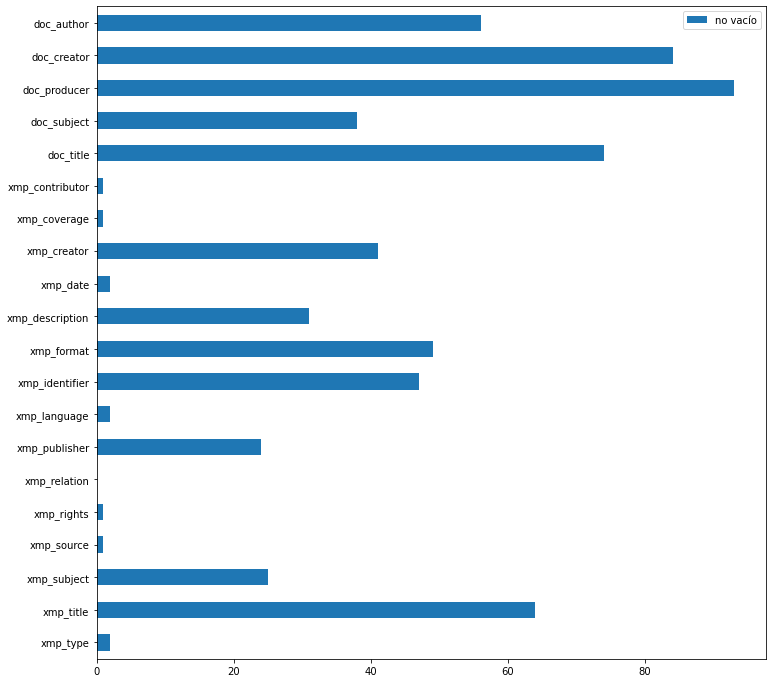
\includegraphics[width=0.9\linewidth]{../images/pdf-metadata-count}
	\caption{Conteo de metadatos incluidos en los PDF}
	\label{fig:pdf-meta-count}
\end{figure}

Tras el proceso de análisis y extracción de metainformación, el resultado de los metadatos no vacíos se muestra en la figura \ref{fig:analytics-meta-count}.

\begin{figure}[h]
	\centering
	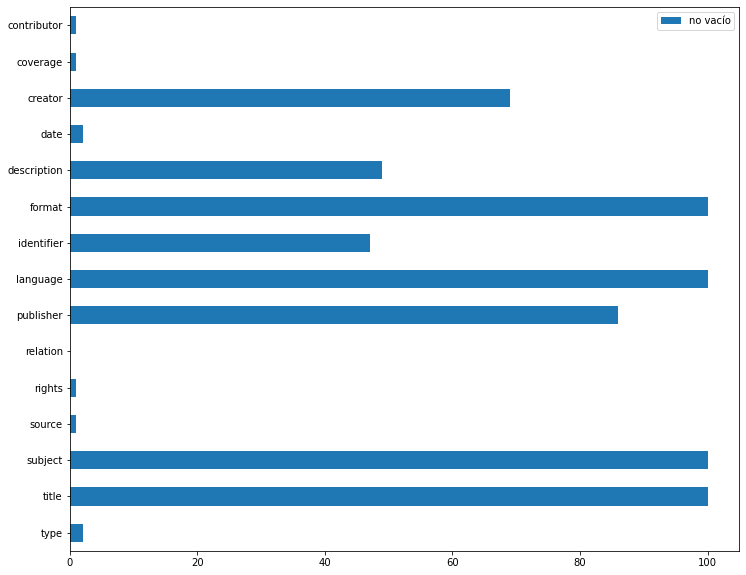
\includegraphics[width=0.9\linewidth]{../images/analytics-metadata-count}
	\caption{Conteo de metadatos tras analizar los artículos}
	\label{fig:analytics-meta-count}
\end{figure}

En las figuras \ref{fig:results-paper-stats}, \ref{fig:results-paper-metadata} y \ref{fig:results-paper-wordcloud} se muestran las salidas de un cuaderno Jupyter para un artículo.

\begin{figure}[h]
	\centering
	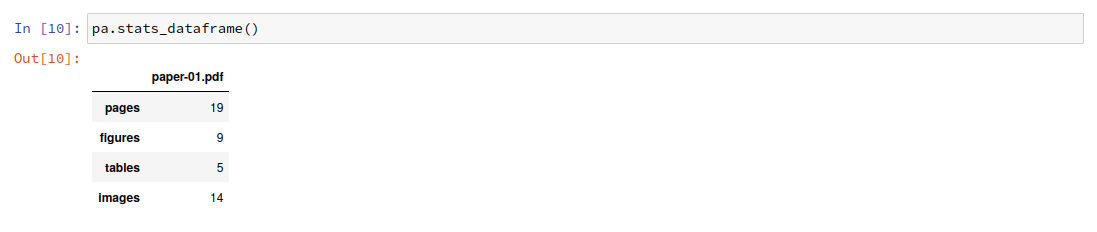
\includegraphics[width=0.9\linewidth]{../images/results-paper-stats}
	\caption{Estadísticas de un artículo en Jupyter}
	\label{fig:results-paper-stats}
\end{figure}

\begin{figure}[h]
	\centering
	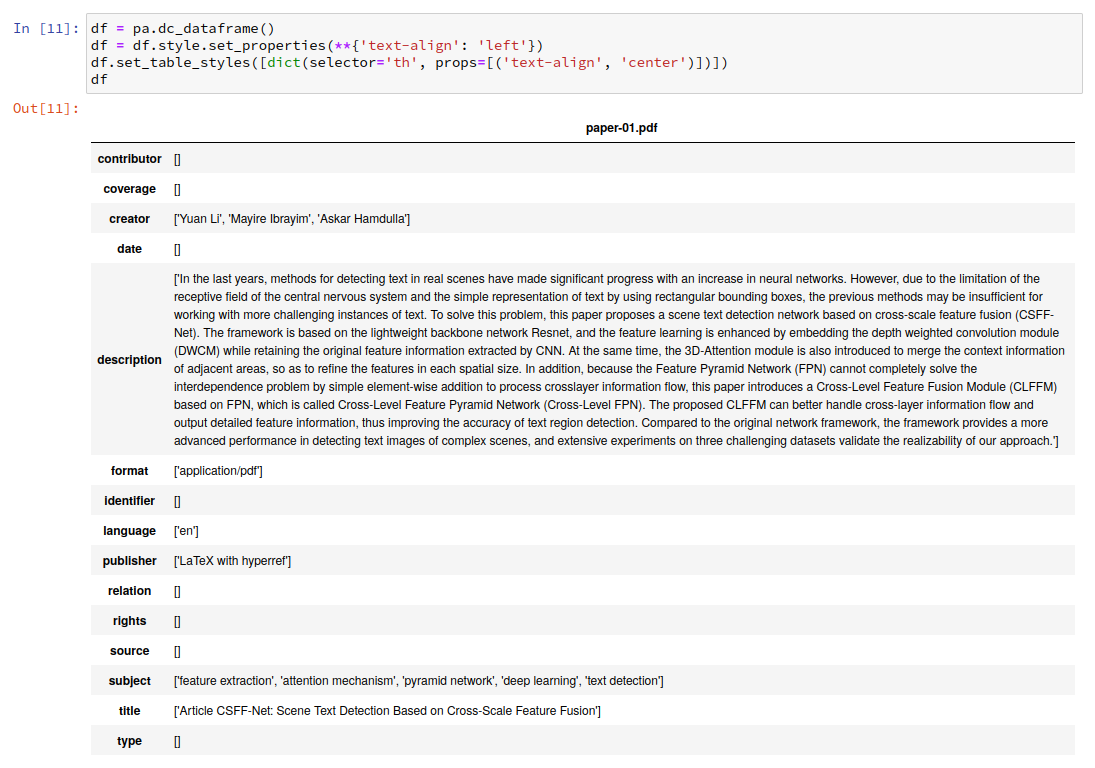
\includegraphics[width=0.9\linewidth]{../images/results-paper-metadata}
	\caption{Metadatos de un artículo en Jupyter}
	\label{fig:results-paper-metadata}
\end{figure}

\begin{figure}[h]
	\centering
	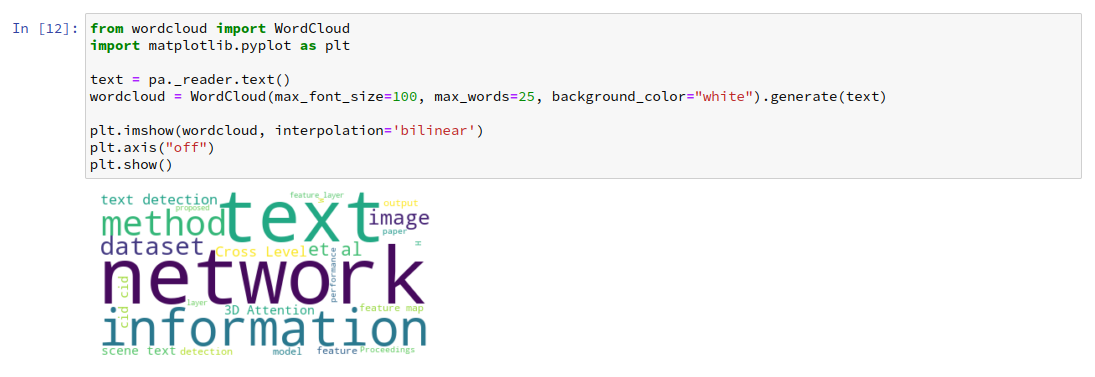
\includegraphics[width=0.9\linewidth]{../images/results-paper-wordcloud}
	\caption{Nube de palabras de un artículo en Jupyter}
	\label{fig:results-paper-wordcloud}
\end{figure}

Por último, en la figura \ref{fig:results-folder-xml} se ve la salida generada en XML con los datos extraídos de todos los artículos del directorio.

\begin{figure}[h]
	\centering
	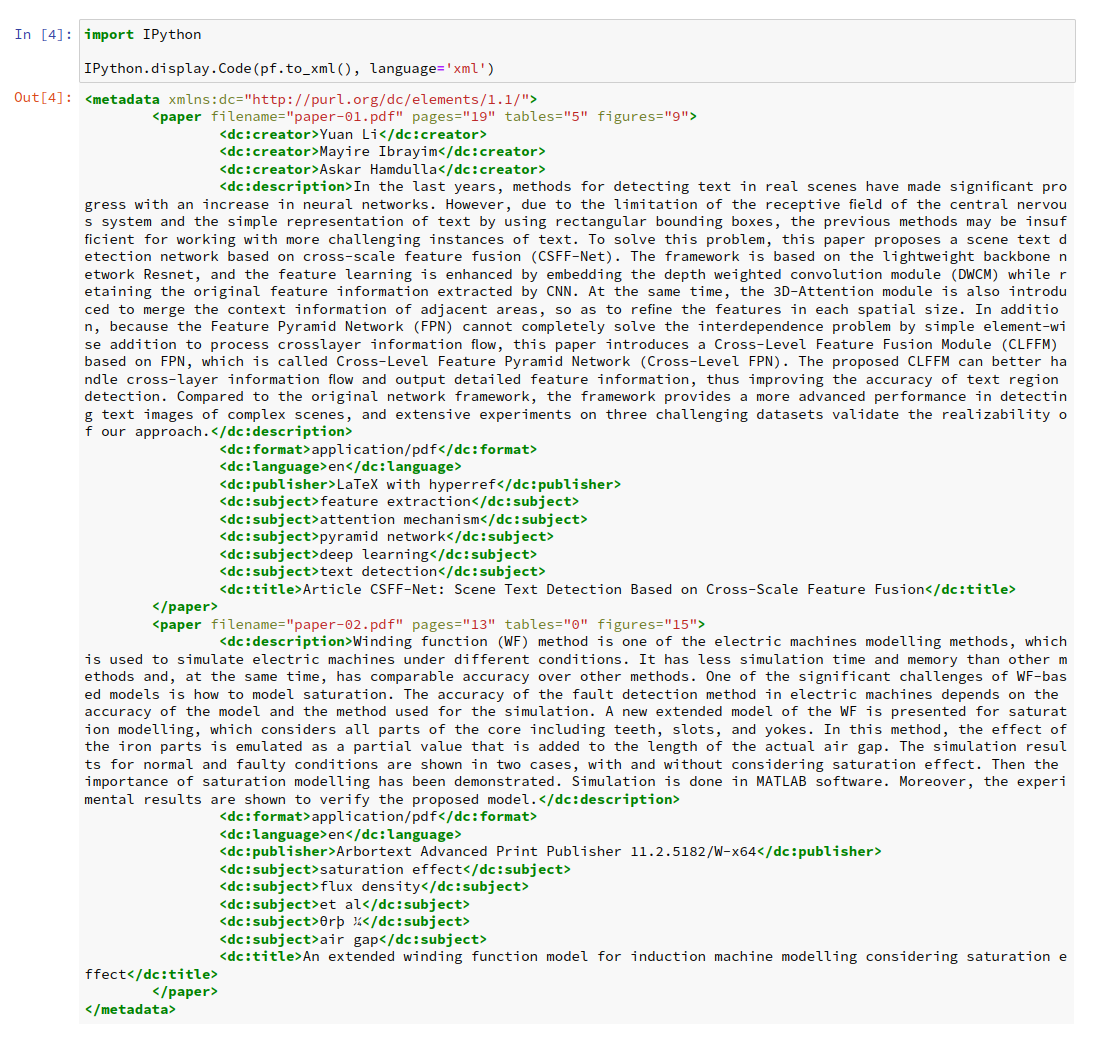
\includegraphics[width=0.9\linewidth]{../images/results-folder-xml}
	\caption{XML del directorio de artículos en Jupyter}
	\label{fig:results-folder-xml}
\end{figure}



\end{document}
